
% %\centerline{MHOA, Monday September 28} % Pas de numérotation
%\addcontentsline{toc}{section}{Introduction} % Ajout dans la table des matières

\section*{Introduction}

 La PG (Programmation Génétique) se classe dans la grande famille des algorithmes évolutionnaires qui s'inspire du paradigme de l'évolution darwinienne afin de faire évoluer des populations de solutions potentielles.
 
 Cette population va subir les différentes étapes d'un processus évolutif simulé :
 
\begin{itemize}
\item sélection des individus les mieux adaptés à leur environnement (dans le cadre de la programmation génétique, cela correspond aux programmes répondant le mieux au problème posé)
\item croisement des individus, dans le cadre de la programmation génétique, ce processus correspond à de "subtiles" échanges de codes entre deux programmes.
\item mutation aléatoire des individus
\end{itemize}
et on veut évoluer un programme afin qu'il résolve un problème donné de façon optimale.

La partie la plus délicate dans les techniques évolutionnaires est l'écriture d'une fonction d'adaptation. Toujours dans le cadre du \textbf{mimétisme} du processus darwinien, seuls les individus les mieux adaptés à leur environnement survivent. Il devient donc nécessaire d'écrire de manière informatique une telle fonction \textit{fitness} qui évaluera les individus (les programmes) afin de leur donner une note qualifiant leur degré d'adaptation.

L'autre écueil, plus spécifique à la programmation génétique consiste à sélectionner les briques de base qui permettront à créer des programmes. Si mon ensemble de brique de base est trop restreint, je ne pourrai peut-être jamais obtenir une solution au problème, par si cet ensemble est trop vaste, le processus algorithmique risque de ne jamais pouvoir converger.

Historiquement, les langages utilisés pour la programmation génétique étaient les langages fonctionnels comme le LISP ou Scheme.

Maintenant, on utilise des langages plus "classiques" comme le langage C, Python, Java, mais également le langage machine pour des raisons de rapidité.\\
\subsection{Attente d'un tel programme}
\begin{itemize}
\item produise un output adéquat pour tous les input possibles.
\item Pour vérifier qu'un programme est bon, on pourrait le
coupler à un simulateur et ajuster le programme pour
minimiser le nombre d'erreur
\item On peut voir cela comme un problème d'apprentissage ou aussi comme un problème d'optimisation : minimiser la différence entre les outputs produits et les outputs spécifiés.
\item Le plus souvent cela consiste à trouver un programme qui
produit des valeurs de sorties données à partir de valeurs
d'entrées données
\item  Les données choisies sont définies comme l'ensemble
d'apprentissage, ou l'ensemble test.
\item Le but est alors que ce programme élaboré sur ce test-set soit
capable de généralisation, c'est à dire qu'il aura capté la
relation sous-jacente et qu'il pourra trouver l'output pour des
inputs nouveaux.

\end{itemize}

\section{Comment faire ?}
\subsection{Codeage par une S-expression}
Koza a proposé de coder un programme avec un langage
fonctionnel, à la Lisp, construit à base d'instructions appelée
S-expressions par exemple comme dans ce TP on a 
\begin{equation}
-2 (\frac{sin(x)}{y})
\end{equation}

qui signifie 
\begin{center}\texttt{2 NEG X SIN Y DIV MUL}
\end{center}
Si on remplace une opérande d'une S-expression par une autre
S-expression, on obtient en général une formule valide, on peut alors définir des opérateurs 
d'évolution génétique qui
mutent ou croisent les S-expressions
\subsection{Function set et Terminal set}
Comme on voit dans le code python, \texttt{functionSet et TerminalSet} ici une petite 
description.\\
Formellement l'espace de recherche des programmes
génétiques est spécifié par un ensemble F de fonctions et un
ensemble T de terminaux. où
\begin{center}
\begin{itemize}
\item F contient les opérations possible dans cet espace
\item T contient les variables et constantes possibles
\item[] For example F = \texttt{And, Or, NOT}
avec des terminaux qui pourraient inclure des variables Booléennes
et des constantes :
T = {b1, b2, b3, . . . , True, False}.
\end{itemize}
\end{center}
\textbf{Note Supp.: on peut définir des opérateurs IF dans le \texttt{function-set}}\\
Par exemple : \texttt{(IF A B C D)} est une fonction à 4 arguments.\\
Si \texttt{A == B} alors \texttt{C} est retourné. Sinon D est retourné.

\subsection{Propriété de clôture}
\begin{itemize}
\item[$ \bullet $] Chaque fonction doit pouvoir accepter comme arguments
toutes les valeurs renvoyées par les autres fonctions, ainsi que
toute valeur appartenante à T.
\item[$ \bullet $] La division, les opérateurs unaires, etc doivent être augmentés
pour accepter n'importe quelle paire d'arguments.
\item[$ \bullet $] L'espace des programmes possibles est formé par toutes les
composition de fonctions possibles à partir des éléments de F
et de T.
\item[$ \bullet $] Cet espace est potentiellement de taille infinie et la longueur des 
individus est arbitraire.
\end{itemize}
\subsection{Crossover}
 L'opération de croisement se fait en sélectionnant un lien au
hasard dans l'arbre représentant chaque parent et en
échangeant les sous-arbres correspondants, comme c'est présenter dans la figure ci dessous, 
et les point de croisement sont d'ordinaire choisis avec probabilité non-uniforme afin de 
favoriser les noeuds
internes par rapport aux feuilles et les parties basses de l'arbre
\begin{figure}[H]
\centering

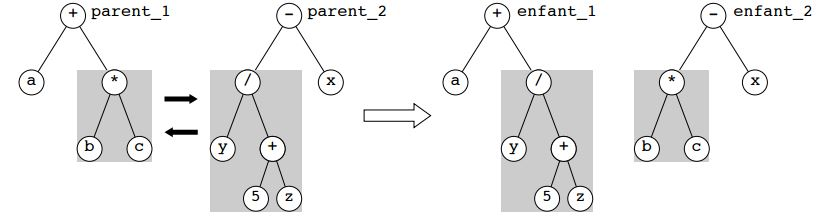
\includegraphics[width=\linewidth]{../figures/codagearbrea.JPG}
\caption{Crossover KOZA}
\label{fig:Crossoverkoza}
\end{figure}
\textbf{\textcolor{red}{Note}}: quand je parle de l'arbre, ça fait référence au codage 
par arbre qui est équivalent à une S-expression mais plus lisible(vue dans le cours)

\subsection{Mutation}
\begin{figure}[H]
\centering
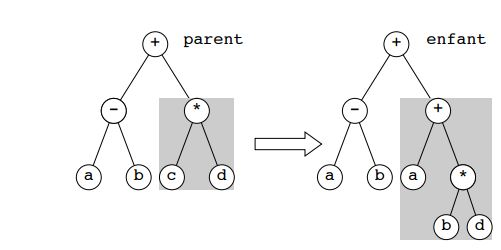
\includegraphics[width=\linewidth]{../figures/codagearbreb.JPG}
\caption{Mutation KOZA}
\label{fig:Mutationkoza}
L’opérateur de mutation est réalisé en sélectionnant de
manière aléatoire un sous-arbre du programme et en lui
substituant un autre sous-arbre et ce dernier est typiquement généré au hasard à partir
des ensembles \textit{F} et \textit{T} du problème.
\end{figure}
\subsection{Projection des concept générale sur ce TP}
Ici on code un PG pqr une suite d'instructions aui seront exécutées sequentiellement.\\
Par exemple:\\ \texttt{}
L'instruction A place la valeur de la variable \textit{A} sur une pile.\\
Les opérations doivent adaptées pour tolérer le manque d'un argument sur la pile\\
L'espace ds programme est donc défini par l'ensemble des instructions possibles, qui 
comprend des variables, constantes et opérations.\\
Pour le \textbf{Crossover} on peut utiliser le crossover à un point vu pour les chaînes 
de bits.\\
Pour la \textbf{mutation}, elle est obtenue en chageant une instruction par une autre 
au hasard.\\
L'output est le sommet de la pule après exécution du programme.

\section{Results}
On prend une pupulation de \texttt{popSize =200} et \texttt{pc=0.1} et\texttt{ pm=0.5}
on obtient les résultats suivant :\\
This is a result for one of the execution with 
$ p_c = 0.6 $, $ p_m = 0.5 $, $ popSize = 200 $
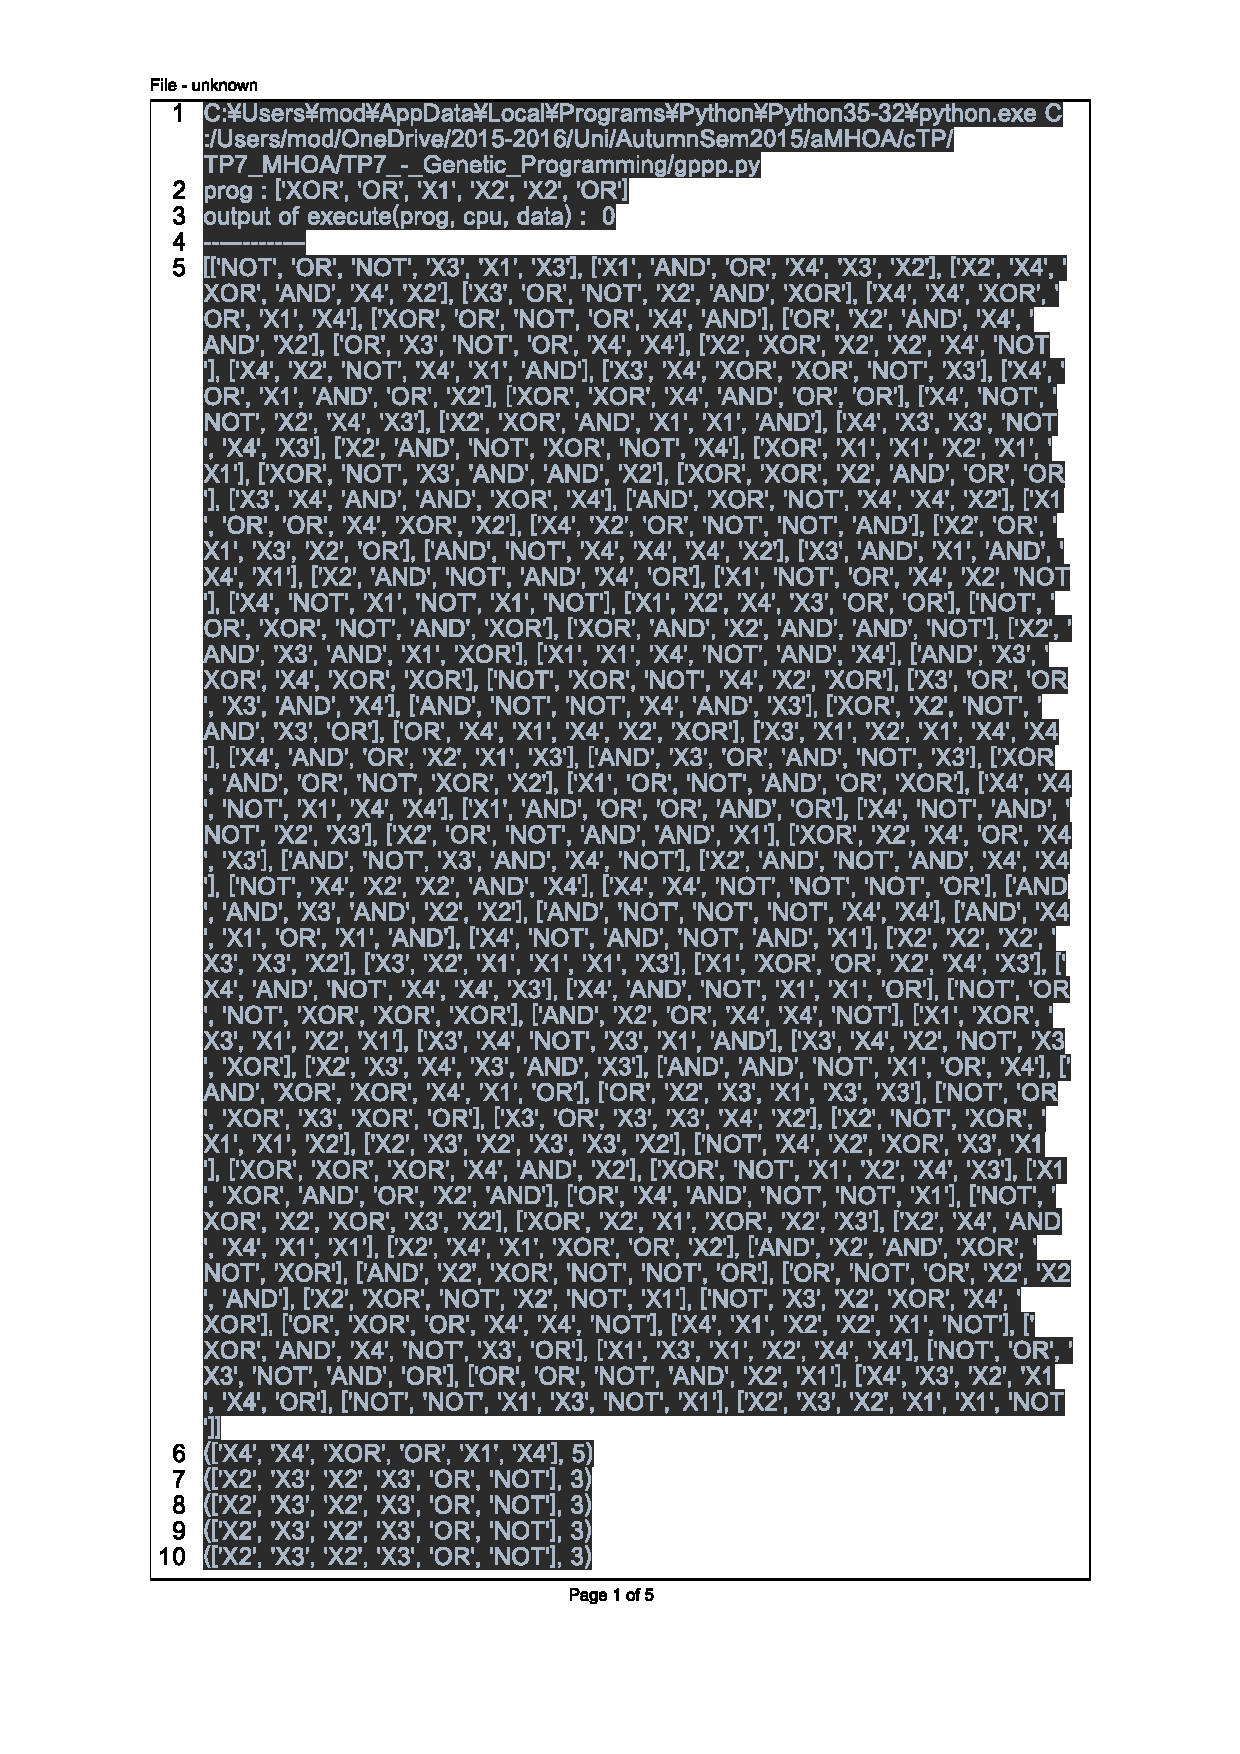
\includepdf[pages={1-},scale=0.75]{../figures/javaprinting.pdf}
Dans cet expérience, on prend une population de 100, qu'on fait évoluer 100 fois avec selection, crossover et mutation, ainsi je fais fixer $ p_c $ et varier $ p_m $ d'une façon croissante.
\begin{table}[H]
{\renewcommand{\arraystretch}{1.2}} 
\centering
\caption{Results with changing parameters of $ p_c\ \&\ p_m $}
\vspace{+5mm}
\label{}
\begin{adjustbox}{width=\linewidth}
\begin{tabular}{|c|c|c|c|c|c|}

\hline
\multicolumn{1}{|c|}{}                                  & \multicolumn{5}{c|}{\texttt{popSize = 100}}                                                                                                                                                                                                                                                                                                                                                                                                                                                                                                                          \\ \hline
\multicolumn{1}{|c|}{\texttt{Res\textbackslash params}} & \multicolumn{1}{c|}{\begin{tabular}[c]{@{}c@{}}$p_c$ = 0.6\\ $p_m$= 0.01\end{tabular}}                         & \multicolumn{1}{c|}{\begin{tabular}[c]{@{}c@{}}$p_c$ = 0.6\\ $p_m$=0.1\end{tabular}}                          & \multicolumn{1}{c|}{\begin{tabular}[c]{@{}c@{}}$p_c$ = 0.6\\ $p_m$=0.2\end{tabular}}                         & \multicolumn{1}{c|}{\begin{tabular}[c]{@{}c@{}}$p_c$ = 0.6\\ $p_m$= 0.4\end{tabular}}                          & \multicolumn{1}{c|}{\begin{tabular}[c]{@{}c@{}}$p_c$ = 0.6\\ $p_m$=0.5\end{tabular}}                          \\ \hline
\multicolumn{1}{|c|}{\texttt{Best F}}                   & \multicolumn{1}{c|}{3.0}                                                                                     & \multicolumn{1}{c|}{3.0}                                                                                    & \multicolumn{1}{c|}{1.0}                                                                                   & \multicolumn{1}{c|}{3.0}                                                                                     & \multicolumn{1}{c|}{3.0}                                                                                    \\ \hline
\multicolumn{1}{|c|}{\texttt{Mean}}                     & \multicolumn{1}{c|}{3.0}                                                                                     & \multicolumn{1}{c|}{3.4}                                                                                    & \multicolumn{1}{c|}{1.48}                                                                                  & \multicolumn{1}{c|}{2.98}                                                                                     & \multicolumn{1}{c|}{3.0}                                                                                    \\ \hline
\multicolumn{1}{|c|}{\texttt{STD}}                      & \multicolumn{1}{c|}{0.0}                                                                                     & \multicolumn{1}{c|}{0.28141058827257937}                                                                                    & \multicolumn{1}{c|}{0.8584693919818557}                                                                    & \multicolumn{1}{c|}{0.2}                                                                                     & \multicolumn{1}{c|}{0.0}                                                                                    \\ \hline
\multicolumn{1}{|c|}{\texttt{}}                         & \multicolumn{1}{c|}{\begin{tabular}[c]{@{}c@{}}{[}'X1', 'X1', 'X2', \\ 'X3', 'X3', 'XOR'{]}\end{tabular}}    & \multicolumn{1}{c|}{\begin{tabular}[c]{@{}c@{}}{[}'X1', 'X2', 'X4',\\  'XOR', 'X4', 'AND'{]}\end{tabular}}  & \multicolumn{1}{c|}{\begin{tabular}[c]{@{}c@{}}{[}'X2', 'X3', 'OR', \\ 'NOT', 'X4', 'AND'{]}\end{tabular}} & \multicolumn{1}{c|}{\begin{tabular}[c]{@{}c@{}}{[}'X1', 'X2', 'X4',\\  'X1', 'X1', 'XOR'{]}\end{tabular}}    & \multicolumn{1}{c|}{\begin{tabular}[c]{@{}c@{}}{[}'XOR', 'X3', 'X4',\\  'OR', 'X3', 'XOR'{]}\end{tabular}}  \\ 
\hline
\end{tabular}

\end{adjustbox}
\end{table}

\subsection{discussion exp 1}
Dans cet expérience ça se voit que la mutation nous faire éviter à s'enliser dans des 
optima locaux. Mais si elle est trop fréquente, le PG est orienté vers une recherche 
aléatoire de la bonne solution.
Dans le tableau ci dessous  on fait la même expérience d'avant mais en variant $ p_c $
\begin{table}[H]

\centering
\caption{Results with varying $ p_c =0.6 $, increasing it}
\label{}
\vspace{+5mm}
\begin{adjustbox}{width=\linewidth}
\begin{tabular}{|c|c|c|c|c|c|}
\hline

\multicolumn{6}{|l|}{}                                                                                                                                                                                                                                                                                                                                                                                                                                                                                                  \\ \hline
\multicolumn{1}{|c|}{}                                  & \multicolumn{1}{c|}{\texttt{popSize = 100}}                                                                  & \multicolumn{1}{c|}{\texttt{popSize = 100}}                                                                              & \multicolumn{1}{c|}{\texttt{popSize = 100}}                                                                             & \multicolumn{1}{c|}{\texttt{popSize = 100}}                                                                               & \multicolumn{1}{c|}{\texttt{popSize = 100}}                                                                              \\ \hline
\multicolumn{1}{|c|}{\texttt{Res\textbackslash params}} & \multicolumn{1}{c|}{\begin{tabular}[c]{@{}c@{}}$p_m$ = 0.6\\ $p_c$= 0.01\end{tabular}}                         & \multicolumn{1}{c|}{\begin{tabular}[c]{@{}c@{}}$p_m$ = 0.6\\ $p_c$=0.1\end{tabular}}                          & \multicolumn{1}{c|}{\begin{tabular}[c]{@{}c@{}}$p_m$ = 0.6\\ $p_c$=0.2\end{tabular}}                         & \multicolumn{1}{c|}{\begin{tabular}[c]{@{}c@{}}$p_m$= 0.6\\ $p_c$= 0.4\end{tabular}}                           & \multicolumn{1}{c|}{\begin{tabular}[c]{@{}c@{}}$p_m$= 0.6\\ $p_c$=0.5\end{tabular}}                           \\ \hline
\multicolumn{1}{|c|}{\texttt{Best F}}                   & \multicolumn{1}{c|}{3.0}                                                                                     & \multicolumn{1}{c|}{3.0}                                                                                    & \multicolumn{1}{c|}{3.0}                                                                                   & \multicolumn{1}{c|}{3.0}                                                                                     & \multicolumn{1}{c|}{1}                                                                                      \\ \hline
\multicolumn{1}{|c|}{\texttt{Mean}}                     & \multicolumn{1}{c|}{4.5}                                                                                     & \multicolumn{1}{c|}{3.08}                                                                                   & \multicolumn{1}{c|}{3.12}                                                                                  & \multicolumn{1}{c|}{3.02}                                                                                    & \multicolumn{1}{c|}{1.62}                                                                                   \\ \hline
\multicolumn{1}{|c|}{\texttt{STD}}                      & \multicolumn{1}{c|}{1.3349989596333858}                                                                      & \multicolumn{1}{c|}{0.3938927711338647}                                                                     & \multicolumn{1}{c|}{0.47736651315188405}                                                                   & \multicolumn{1}{c|}{0.2}                                                                                     & \multicolumn{1}{c|}{0.9296463974234636}                                                                     \\ \hline
\multicolumn{1}{|c|}{\texttt{}}                         & \multicolumn{1}{c|}{\begin{tabular}[c]{@{}c@{}}{[}'NOT', 'XOR', 'X4',\\  'AND', 'X4', 'XOR'{]}\end{tabular}} & \multicolumn{1}{c|}{\begin{tabular}[c]{@{}c@{}}{[}'X2', 'AND', 'X2',\\  'XOR', 'OR', 'XOR'{]}\end{tabular}} & \multicolumn{1}{c|}{\begin{tabular}[c]{@{}c@{}}{[}'X3', 'XOR', 'X3',\\ 'NOT', 'X4', 'AND'{]}\end{tabular}} & \multicolumn{1}{c|}{\begin{tabular}[c]{@{}c@{}}{[}'AND', 'X4', 'XOR', \\ 'X4', 'XOR', 'XOR'{]}\end{tabular}} & \multicolumn{1}{c|}{\begin{tabular}[c]{@{}c@{}}{[}'X4', 'X3', 'X2', \\ 'NOT', 'XOR', 'AND'{]}\end{tabular}} \\  
\hline

\end{tabular}

\end{adjustbox}
\end{table}

\subsection{discussion exp 2}
Après regarder les résultat comme dans la page -5-6-7 pour chaque exécution on 
remarque bien que s'il n'y a pas de crossover où la valeur très proche de zero, 
les nouvelles générations sont l'exacte copie des racines alors que s'il y a du crossover, 
les générations sont composés d'une partie de chacun de leur racines et alors les nouveaux 
générations gardent la meilleur partie des  anciens.et si la probabilité est au max tous les 
descendant sont générés par crossover\\Ceci dans le but d'obtenir de meilleurs générations. 
néanmoins, il est quand même important qu'une partie de la population survivre à la nouvelle 
génération.


Dans cet expérience, on prend une population de 12, qu'on
fait évoluer 50 fois avec selection, crossover et mutation.

\begin{table}[H]

\centering
\caption{Results with same params $ P_m = 0.01 $, $ p_c =0.6 $ on 5 execution}
\label{}
\vspace{+5mm}
\begin{adjustbox}{width=\linewidth}
\begin{tabular}{|c|c|c|c|c|c|}
\hline
       & \multicolumn{5}{c|}{popSize = 12}                                                                                                                                                                                                                                                                                                                                                                                                                      \\ \hline
Exec   & 1                                                                                     & 2                                                                                     & 3                                                                                      & 4                                                                                    & 5                                                                                      \\ \hline
Best F & 1.0                                                                                   & 3.0                                                                                   & 3.0                                                                                    & 3.0                                                                                  & 1                                                                                      \\ \hline
Mean   & 1.06                                                                                  & 3.02                                                                                  & 3.56                                                                                   & 3.04                                                                                 & 1.69                                                                                   \\ \hline
STD    & 0.3428932159955306                                                                    & 0.2                                                                                   & 0.282842712474619                                                                      & 0.282842712474619                                                                                 & 0.3938927711338647                                                                                   \\ \hline
       & \begin{tabular}[c]{@{}c@{}}{[}'X4', 'X3', 'X2', \\ 'OR', 'NOT', 'AND'{]}\end{tabular} & \begin{tabular}[c]{@{}c@{}}{[}'OR', 'NOT', 'X3',\\  'OR', 'X3', 'XOR'{]}\end{tabular} & \begin{tabular}[c]{@{}c@{}}{[}'X2', 'XOR', 'AND',\\  'OR', 'XOR', 'X4'{]}\end{tabular} & \begin{tabular}[c]{@{}c@{}}{[}'OR', 'X4', 'XOR',\\ 'X4', 'OR', 'XOR'{]}\end{tabular} & \begin{tabular}[c]{@{}c@{}}{[}'NOT', 'X3', 'X2',\\  'NOT', 'X4', 'AND'{]}\end{tabular} \\ \hline
\end{tabular}

\end{adjustbox}
\end{table}

\subsection{discussion exp 3}
J'ai fait cet expérience pour voir l'effet du size de la population sur les résultats et comme
présent dans le tableau ci dessus, on remarque que le STD varie d'autant que dans les premiers 
deux expérience avec un optimum de 1 où la $ p_c= 0.01 $ et $ p_c = 0.5 $ alors que 
pour $ p_c$ > 0.1 et <0.5 le meilleur optimum est 3 et l'écart type est respectivement 
autour de 34\% et 20 \%
\section{Conclusion et discussion générale}
Durant toutes les expériences on ne trouve pas l'optimum à chaque run, et donc l'optimum 
a fitness 1.\\
Il y a des fonction qui sont curieusement plus difficile à trouve car l'une des éléments 
du programme est un attracteur.\\

Les algorithmes génétiques fournissent des solutions proches de la solution optimale à 
l'aide des mécanismes de sélection, de crossover et de mutation comme le montre les 3 
tableau ci dessus. et c'est pour ça qu'ils sont applicables à nombreux problèmes, dont 
le problème de vol (crach vol \~ erreur).\\
Une note sur la méthode de séléction par tournoi, c'est que avec un nombre élevé de 
participant, un individu faible sera presque toujous sûr de perdre.\\

Finalement avec cette méthode on peut trouves des programmes qui répondes au mueux 
à une tache définie. Pour ce faire, elle permet à la machine d'apprendre, en utilisant 
cet algorithme évolutionniste afin d'optimiser la population de programmes.

